\begin{chapter}{\label{cha:numerics}Numerical Theory and Procedures}
\section{\label{section:RK} Numerical procedures for 2D and 3D solutions}
	\subsection{\label{section:RK4} Fourth order Runge-Kutta scheme}
	The classical fourth-order Runge-Kutta formula (RK4) is described equivalently in many texts. We follow the description in \cite{NumericalRecipes}. Let an initial value problem be specified as
	
	\begin{align*}
		\frac{\partial \psi}{\partial t} &= f(\psi,t),\hspace{0.25in}\psi(t_0) = \psi_0.
	\end{align*}

A step-size, $h>0$, is chosen as the parameter controlling how the solution is advanced over $t$. The scheme for estimating $\psi(t_n)= \psi_n$ is then written
\begin{equation}
\begin{split}
		k_1 &= hf(t_n,\psi_n),\\
		k_2 &= hf(t_n+\frac{h}{2},\psi_n+\frac{k_1}{2}),\\
		k_3 &= hf(t_n+\frac{h}{2},\psi_n+\frac{k_2}{2}),\\
		k_4 &= hf(t_n+h,\psi_n+k_3),\\
		\psi_{n+1} &= \psi_n + \frac{k_1}{6}+ \frac{k_2}{3}+ \frac{k_3}{3} + \frac{k_4}{6} + \mathcal{O}(h^5),\\
		t_{n+1}  &= t_n + h.
		\label{eq:rk4}
\end{split}
\end{equation}


	An outline derivation of the Runge-Kutta scheme, which includes a proof of accuracy are shown in Appendix \ref{appsection:rk4deriv}.
	In all of our relevant calculations the value of f is set as the right hand side of the homogeneous or trapped GPE. The main loop formulating the RK4 method may be repeated indefinitely to reach any $t>t_0$. The step size for a given set of parameters should be chosen small enough that smaller choices make no quantitative changes to the resulting solution. The following section outlines the methods we have implemented to ensure numerical solutions are converged.

	\subsection{\label{section:numericalParams} Numerical stability and convergence}
	We now investigate numerical parameters which affect the stability of simulated superfluid systems. Our direct aim is to find a suitable discretisaton of space and time so that while simulations are timely, our numerical quantities are converged (so that they are not sensitive to small changes in computational parameters) and that quantities conserved by the equations of motion are indeed conserved in the computed numerical solutions.

	We begin by estimating $\Delta_x$, the required spatial grid spacing, by considering the width of the vortex core in a homogeneous system, a feature we would like well and accurately visualised in our numerical solutions. Through observation of a singly quantised vortex core (as in Figure \ref{fig_vortex}) we observe a core radius of approximately $5\xi$ when the background density is $\rho=1$. To ensure the vortex core structure is well resolved we decide to dedicate 10 grid points for a vortex core radius, suggesting a value of $\Delta_x = \xi/2$.

	In the trapped case we can use the same idea. It is shown in Section \ref{section:healing} that $\xi = \hbar/\sqrt{mg}$ for $\rho=1$. We can then easily rearrange to find an expression for $\xi$ in the harmonic oscillator units of trapped condensates. We find that our approximate grid spacing to adequately resolve the vortex core is $\Delta_x = 0.5\xi = 0.5\omega \sqrt{\hbar/(\mu \omega)} l_r$. As an example, for a trapped condensate with interaction energy $\hat{g}=2000$, chemical potential $\hat{\mu}=25.27$ and trap frequency $\omega=8.75~{\rm Hz}$ we find that a value of $\Delta_x=0.1l_r$ should be adequate. 

	Similar arguments (concerned with time rather than space), can be used to approximate a suitable time step $h$. We define a time period that we would like to be well resolved by considering by the smallest possible element moving at the fastest reasonable speed. If we define this period as $\Delta_x / 5~c$ and allocate to it 10 time steps, we find that $h = 0.5\xi/50~c = 0.01\tau$.

  In addition to this process, for each set of simulation parameters it is recommended to confirm the suitability of the chosen $\Delta_x$ and $h$ by testing the convergence and conservation in the numerical methods. The total condensate energy and particle number are good measures for this as they should both be well conserved by the GPE with a dissipation of $\gamma=0$. An example of this process (confirming the suitability of a chosen $\Delta_x$) is shown in Figure \ref{fig_energ_norm_cons}: For a large $\Delta_x=0.4l_r$ both the condensate energy and norm fluctuate wildly. For $\Delta_x=0.1l_r$ the norm is extremely well conserved to within $2.10^{-5}\%$ and the energy is conserved within $5.10^{-3}\%$. The smallest tested value of $\Delta_x=0.05l_r$ finally confirms that the energy has converged. We conclude that for the chosen system parameters that $\Delta_x=0.1l_r$ (the value suggested by the above analysis) is numerically sufficient and there is little reason to use $\Delta_x<0.1l_r$.

  \begin{figure}
  \centering
   \begin{tikzpicture}
    \begin{axis}[y tick label style={
            /pgf/number format/.cd,
                fixed,
                fixed zerofill,
                precision=3,
            /tikz/.cd
        },
        width=0.98\linewidth,
        height=0.3\linewidth,
        xlabel={},
        ylabel=$\hat{E}\left ( \hat{t} \right )$,
        xmin=0,
        xmax=10,
        major tick length = 0.07cm
      ]
      \addplot gnuplot [raw gnuplot,mark=none,color=black,thick]{
        plot "numerics/figures/energ-norm-cons.0.05" using 1:3 with lines;
      };
      \addplot gnuplot [raw gnuplot,mark=none,color=red,thick]{
        plot "numerics/figures/energ-norm-cons.0.1" using 1:3 with lines;
      };
      \addplot gnuplot [raw gnuplot,mark=none,color=green,thick]{
        plot "numerics/figures/energ-norm-cons.0.2" using 1:3 with lines;
      };
      \addplot gnuplot [raw gnuplot,mark=none,color=blue,thick]{
        plot "numerics/figures/energ-norm-cons.0.4" using 1:3 with lines;
      };
    \end{axis}
  \end{tikzpicture}
  \begin{tikzpicture}
    \begin{axis}[y tick label style={
            /pgf/number format/.cd,
                fixed,
                fixed zerofill,
                precision=4,
            /tikz/.cd
        },
        width=0.98\linewidth,
        height=0.35\linewidth,
        name=mainplot,
        xlabel=$\hat{t}$,
        ylabel=$\hat{N}\left ( \hat{t} \right )$,
        xmin=0,
        xmax=10,
        ymax=1.0008,
        major tick length = 0.07cm
      ]
      \addplot gnuplot [raw gnuplot,mark=none,color=black,thick]{
        plot "numerics/figures/energ-norm-cons.0.05" using 1:4 with lines;
      };
      \addplot gnuplot [raw gnuplot,mark=none,color=red,thick]{
        plot "numerics/figures/energ-norm-cons.0.1" using 1:4 with lines;
      };
      \addplot gnuplot [raw gnuplot,mark=none,color=green,thick]{
        plot "numerics/figures/energ-norm-cons.0.2" using 1:4 with lines;
      };
      \addplot gnuplot [raw gnuplot,mark=none,color=blue,thick]{
        plot "numerics/figures/energ-norm-cons.0.4" using 1:4 with lines;
      };
      \node[anchor=west] (source) at (axis cs:9.25,1.00027){};
      \node[anchor=west] (destination) at (axis cs:9.25,1.0000){};
      \node[anchor=west] (topl) at (axis cs:9.2,1.00005){};
      \node[anchor=west] (botr) at (axis cs:9.8,0.99995){};
      \draw[->](source)--(destination);
      \draw(topl) rectangle (botr);
    \end{axis}
    \begin{axis}[y tick label style={
            /pgf/number format/.cd,
                fixed,
                fixed zerofill,
                precision=6,
            /tikz/.cd
        },
        width=0.35\linewidth,
        height=0.18\linewidth,
        at={(mainplot.north east)},anchor=north east,
        xlabel={},
        ylabel={},
        xmin=9.15,
        xmax=9.85,
        major tick length = 0.07cm
      ]
      \addplot gnuplot [raw gnuplot,mark=none,color=black,thick]{
        plot "numerics/figures/energ-norm-cons.0.05" using 1:4 with lines;
      };
      \addplot gnuplot [raw gnuplot,mark=none,color=red,thick]{
        plot "numerics/figures/energ-norm-cons.0.1" using 1:4 with lines;
      };
      \addplot gnuplot [raw gnuplot,mark=none,color=green,thick]{
        plot "numerics/figures/energ-norm-cons.0.2" using 1:4 with lines;
      };
    \end{axis}
  \end{tikzpicture}
  \caption{Dimensionless energy, $\hat{E}$, and particle number, $\hat{N}$, throughout numerical propagation of a trapped condensate containing a singly quantised vortex in its center, with interaction energy $\hat{g}=2000$ and chemical potential $\hat{\mu}=25.27$. The numerical grid width varies with each line; $\Delta_x = 0.05$ (black), $\Delta_x = 0.1$ (red), $\Delta_x = 0.2$ (green) and $\Delta_x = 0.4$ (blue). (Inset) Zoomed view of the $\hat{N}$.}\label{fig_energ_norm_cons}
 \end{figure}

\section{\label{section:vortexidentifying} Identifying vortices}
Large potions of this thesis are dedicated to the study of 2D vortex dynamics. As such, accurate detection of the location and charge of densely packed quantised 2D vortices is required, and so we have developed robust numerical methods for vortex identification. The basic idea is fairly simple, with arguments similar to those used to demonstrate the quantised nature of the circulation.

As shown in Section \ref{section:quantisedcirculation}, the integrated change of phase along any closed curve $C$ is,
\begin{equation}
  \Delta\theta(C) = \oint_C \! \nabla \theta  \, \mathrm{d}\mathbf{l} = 2\pi q,
\end{equation}
where $\mathrm{d}\mathbf{l}$ is the line element and $q\in\mathbb{Z}$. Further, the fundamental theorem of calculus for line integrals[CITE] implies that $\Delta\theta(C) = 0$, providing that $C$ is continuous and does not encompass a phase singularity. This result is crucial; it allows us to directly state that a vortex lies within $C$ if and only if $|\Delta\theta(C)| > 0 $.

\subsection{\label{section:vortexloc} Basic vortex detection method}
First define a set of curves $C_k$ with each curve lying on points of our numerical grid, so that a single $C_k$ encompasses only a small region of the fluid (ideally, $C_k$ should encompass a region at most the diameter of a vortex core). $\Delta\theta(C_k)$ is then approximated for each $k$ using numerical differentiation (2nd order finite differences) and numerical line integration (trapezium or Simpson rule). If $\Delta\theta(C_k) = 0$ to within numerical accuracy then we determine that the region inside $C_k$ contains no vortices. Otherwise the sign of $\Delta\theta(C_k)$ tells us the polarity of the encompassed vortex.

In principle the result also allows us to calculate the exact charge of a vortex in terms of the quantum of circulation. However, for accurate determination of vortex location the curves $C_k$ must encompass a very small area, contain few grid points, and so accuracy is low. We use only the sign of the $\Delta\theta(C_k)$ so that the integration error makes minimal difference and results in an accurate detection of vortex polarity and location. As multiply charged ($|q|>1$) vortices are unstable (rapidly decaying into several singly charged vortices) there is no significant loss of information in practise.
\begin{figure}
  \centering
   \begin{tikzpicture}[
        %>={Straight Barb[left]},
      myarrow/.style={
        decoration={
          markings,
          mark=at position 0.5 with {\arrow{>}};
          },
        postaction=decorate  
        }
      ]
      \begin{axis}[
        xlabel={$x/\xi$},
        ylabel={$y/\xi$},
        x=1cm/4,
        y=1cm/4,
        xmin=-10,
        xmax=10,
        ymin=-10,
        ymax=10,
        colorbar style={title={Phase},text width=0.5em,major tick length = 0.07cm},
        major tick length = 0.07cm,
        point meta min = -3.1415,
        point meta max = 3.1415,
        colorbar,colormap name=hsvcl
      ]
      \addplot graphics [xmin=-10,xmax=10,ymin=-10,ymax=10] {numerics/figures/vortex1dp-hsv.png};
    \end{axis}
      \draw[step=1cm,gray,very thin] (0,0) grid (5,5);
      \foreach \i in {1,...,5}{
        \foreach \j in {1,...,5}{
          \draw [myarrow,thick] (\i-0.07,5.93-\j)--(\i-0.93,5.93-\j);
          \draw [thick] (\i-0.93,5.93-\j)--(\i-0.93,5.07-\j);
          \draw [thick] (\i-0.93,5.07-\j)--(\i-0.07,5.07-\j);
          \draw [thick] (\i-0.07,5.03-\j)--(\i-0.07,5.93-\j);
          {\pgfmathtruncatemacro{\label}{((\j-1)*5) + \i}
          \node[] (c0) at (\i-0.5,5.5-\j) {$C_{\label}$};}
        }
      }
  \end{tikzpicture}
  \caption{The phase for a homogeneous system with a vortex located at (0,0). Also shown is an example set of curves $C_k$ for vortex identification. All $\Delta\theta(C_{k\neq13})\approx0$, and $\Delta\theta(C_{13})>0$. The conclusion is that a positive vortex lies in the region defined by $C_{13}$.}
 \end{figure}
\subsection{\label{section:vortexloc} Visualising vortex location with a vortex field}
The basic vortex identification method set out in Section \ref{section:vortexloc} is quick to implement and useful when there are few well separated vortices, but one can easily imagine a situation where the system fails. One such case would be two vortices both lying within a single $C_k$ curve; in the case of two similarly charged vortices only a single vortex would be detected or in the case of two oppositely charged vortices potentially none at all!

The solution is not always as simple as reducing the size of $C_k$, vortices can be densely packed and there are often too little grid points to make this reasonable. Instead, curves with a width around the diameter of a vortex core are again used, but for every grid point (taking into account boundary conditions) the curve $C_{[i,j]}$ is defined surrounding and centred on the grid point $[i,j]$. A vortex field can then be visualised by visualizing the 2D plot of $\Delta\theta(C_{[i,j]})$. Algorithm \ref{algo_calcvortexfield} describes the process in detail. As before, areas where $|\Delta\theta(C_{[i,j]})| > 0$ (to within numerical accuracy) signify the presence of a vortex. Figure \ref{fig:vortexfield} demonstrates a vortex field obtained from a homogeneous system with a negative vortex located at $(-\xi,0)$ and a positive vortex located at $(\xi,0)$. It can be easily seen where the two vortices are located in the wavefunction by direct observation of the 2D vortex field.
\begin{figure}
  \centering
   \begin{tikzpicture}
      \begin{axis}[
        xlabel={$x/\xi$},
        ylabel={$y/\xi$},
        width=0.45\linewidth,
        height=0.45\linewidth,
        xmin=-10,
        xmax=10,
        ymin=-10,
        ymax=10,
        colorbar style={title={Vortex Field},text width=0.5em,major tick length = 0.07cm},
        major tick length = 0.07cm,
        point meta min = -6,
        point meta max = 6,
        colorbar,colormap/jet
      ]
      \addplot graphics [xmin=-10,xmax=10,ymin=-10,ymax=10] {numerics/figures/v-av-pair-vortexfield.png};
      \addplot[mark=.] coordinates {(-1,0)} node[pin={[pin edge={black,thick}]left:{$1$}}]{} ;
      \addplot[mark=.] coordinates {(1,0)} node[pin={[pin edge={black,thick}]right:{$2$}}]{} ;
    \end{axis}
    
  \end{tikzpicture}
  \caption{Vortex field for two oppositely charged vortices located at ($-\xi$,0) and ($\xi$,0) in a homogeneous system. The positive (negative) vortex leads to a positive (negative) quantity in the vortex field. In addition, the output of the bwlabel algorithm is labelled.\label{fig:vortexfield}}
 \end{figure}

For every vortex detected by this algorithm, the corresponding area in the vortex field is composed of several adjoined points in the numerical grid. For correct vortex counting, these multiple points must be classified as a single vortex. The bwlabel algorithm described in Algorithm \ref{algo_bwlabel} is used to obtain this required classification. The algorithm takes the vortex field as input and assigns each connected component a label. An example output of bwlabel is shown in Figure \ref{fig:vortexfield}. To find the vortex location for a given label, we simply take the mean of all the $x$ and $y$ locations of points with the same label.

The algorithm described in this section leads to more accurate vortex counts when vortices are densely packed. As a bonus the accuracy of detected vortex location is improved; the final output is a combination of information from several curves $C_{[i,j]}$, and so in good conditions the result is often sub-pixel accurate (that is, the algorithm output is accurate even if the phase singularity corresponding to a vortex lies between grid points). 

\subsection{\label{section:gaussianblur} Further improving accuracy with a Gaussian blur}
When using Algorithm \ref{algo_calcvortexfield} in `messy' wavefunctions (containing many vortices and waves), artefacts of the incorrect sign can be introduced by the numerical discretisation, differentiation and integration errors. Faint examples of these artefacts can be seen in Figure \ref{fig:vortexfield} surrounding the two labelled regions. These artefacts are spatially small (on the scale of $\Delta_x$) and so can be corrected by removing all high frequency spatial waves from the vortex field using low-pass filtering. A common low-pass filter is the Gaussian blur [CITE], applied using a convolution. The Gaussian blur algorithm is described in Algorithm \ref{algo_gaussconv} and the result of applying the algorithm to he vortex field is shown in Figure \ref{fig:vortexfieldsmooth}. Note how the incorrectly signed artefacts surrounding the detected vortex regions are now removed.
\begin{figure}[!ht]
  \centering
   \begin{tikzpicture}
      \begin{axis}[
        xlabel={$x/\xi$},
        ylabel={$y/\xi$},
        width=0.45\linewidth,
        height=0.45\linewidth,
        xmin=-10,
        xmax=10,
        ymin=-10,
        ymax=10,
        colorbar style={title={Vortex Field},text width=0.5em,major tick length = 0.07cm},
        major tick length = 0.07cm,
        point meta min = -5.1,
        point meta max = 5.1,
        colorbar,colormap/jet
      ]
      \addplot graphics [xmin=-10,xmax=10,ymin=-10,ymax=10] {numerics/figures/v-av-pair-vortexfield-smoothed.png};
    \end{axis}
  \end{tikzpicture}
  \caption{Smoothed vortex field for two oppositely charged vortices located at ($-\xi$,0) and ($\xi$,0) in a homogeneous system. The high frequency noisy artefacts in the vortex field are removed by the low-pass filtering.\label{fig:vortexfieldsmooth} }
 \end{figure}

 A by-product of applying a low-pass filter to the vortex field is that sharp edges in structures are blurred and spread out. To identify vortex locations a threshold function is therefore used before performing the bwlabel algorithm, i.e vortices are identified when $|\Delta\theta(C_{[i,j]})| > \Delta_{\rm th}$, where $\Delta_{\rm th}>0$ is some threshold. $\Delta_{\rm th}$ can be tweaked to make the vortex detection more or less sensitive (for either detecting vortices more easily in messy systems, or to ignore weak spurious signals in the vortex field) and in general will vary for each system.
\subsection{\label{section:ghostvortex} Avoiding `ghost vortices'}
A common problem when detecting vortices is the prevalence of invalid or uninteresting phase defects inside obstacles or when considering trapped condensates. In areas where the density is exactly zero the system phase becomes undefined. Depending on how the simulation is implemented these areas may fill with small numerical noise and cause many singularities to be detected. A similar phenomenon occurs in areas of near-zero density; well-defined singularities in the phase form but with an ill-defined vortex core in the density \cite{tsubota_kasamatsu_02}. Examples of these vortices are shown in the low density regions of Figure \ref{fig:ghostvortex}. As these singularities carry negligible angular momentum and energy they are of no interest and are termed `ghost vortices'.
\begin{figure}[!ht]
  \centering
   \begin{tikzpicture}
      \begin{axis}[
        xlabel={$x/l_r$},
        ylabel={$y/l_r$},
        width=0.44\linewidth,
        height=0.44\linewidth,
        xmin=-25,
        xmax=25,
        ymin=-25,
        ymax=25,
        major tick length = 0.07cm
      ]
      \addplot graphics [xmin=-25,xmax=25,ymin=-25,ymax=25] {numerics/figures/vortexlatticedens.png};
    \end{axis}
  \end{tikzpicture}
  \begin{tikzpicture}
      \begin{axis}[
        xlabel={$x/l_r$},
        ylabel={},
        width=0.44\linewidth,
        height=0.44\linewidth,
        xmin=-25,
        xmax=25,
        ymin=-25,
        ymax=25,
        colorbar style={title={Phase},text width=0.5em,major tick length = 0.07cm},
        major tick length = 0.07cm,
        point meta min = -3.141592,
        point meta max = 3.141592,
        colorbar,colormap name=hsvcl
      ]
      \addplot graphics [xmin=-25,xmax=25,ymin=-25,ymax=25] {numerics/figures/vortexlatticephase.png};
    \end{axis}
  \end{tikzpicture}
  \caption{A trapped rotating condensate with $\Omega=0.7$, $\hat{g}=2000$ and $\hat{\mu}=25.27$. Ghost vortices can be seen in the phase as singularities where the corresponding density is near-zero.\label{fig:ghostvortex}}
 \end{figure}

A simple way to remove ghost vortices is to use a mask to hide vortices found in low-density regions in trapped systems and inside obstacles. While on the one hand it is easy to define a mask using the TF radius or considering where $V_{\rm trap} + V_{\rm obj}>1$, masks are quite arbitrary in nature and an overzealous mask may hide details. Additionally, any condensate with certain excitations such a breathing mode or centre of mass oscillation will periodically extend beyond a hard coded mask.

An alternative method to avoid identifying ghost vortices presents itself when implementing Algorithm \ref{algo_calcvortexfield}. The vortex field can be multiplied by the wavefunction density at every point {\it before} performing the Gaussian convolution step. The result is that in low-density areas the vortex field becomes completely zero and singularities in this region are no longer identified as vortices. At the centre of vortex cores the vortex field also goes to zero. However, enough vortex information remains in the vortex field in the vicinity of the vortex cores that vortices in high-density regions are still identified accurately after the Gaussian convolution. As before, the threshold value $\Delta_{\rm th}$ controls the sensitivity of this algorithm, in particular for detecting vortices in the low density regions of the condensate. Algorithm \ref{algo_calcvortexfielddens} describes this method in further detail and Figure \ref{fig:filtervortexlattice} shows the vortex field with and without the added step of multiplying by the density, demonstrating that the ghost vortices detected when using Algorithm \ref{algo_calcvortexfield} are indeed removed when using Algorithm \ref{algo_calcvortexfielddens}.
\begin{figure}[!ht]
\begin{center}
\begin{minipage}{0.8\linewidth}%
   \begin{tikzpicture}
      \begin{axis}[
        xlabel={},
        ylabel={$y/l_r$},
        width=0.5\linewidth,
        height=0.5\linewidth,
        xmin=-25,
        xmax=25,
        ymin=-25,
        ymax=25,
        major tick length = 0.07cm
      ]
      \addplot graphics [xmin=-25,xmax=25,ymin=-25,ymax=25] {numerics/figures/vortexlattice-vortexfield.png};
    \end{axis}
  \end{tikzpicture}%
  \begin{tikzpicture}
      \begin{axis}[
        xlabel={},
        ylabel={},
        width=0.5\linewidth,
        height=0.5\linewidth,
        xmin=-25,
        xmax=25,
        ymin=-25,
        ymax=25,
        colorbar style={title={Vortex Field},text width=0.5em,major tick length = 0.07cm},
        major tick length = 0.07cm,
        point meta min = -5.1,
        point meta max = 5.1,
        colorbar,colormap/jet
      ]
      \addplot graphics [xmin=-25,xmax=25,ymin=-25,ymax=25] {numerics/figures/vortexlattice-vortexfield-corrected.png};
    \end{axis}
  \end{tikzpicture}\\\vspace{1cm}%
  \begin{tikzpicture}
      \begin{axis}[
        xlabel={$x/l_r$},
        ylabel={$y/l_r$},
        width=0.5\linewidth,
        height=0.5\linewidth,
        xmin=-25,
        xmax=25,
        ymin=-25,
        ymax=25,
        major tick length = 0.07cm
      ]
      \addplot graphics [xmin=-25,xmax=25,ymin=-25,ymax=25] {numerics/figures/vortexlatticedens-withGvortex.png};
    \end{axis}
  \end{tikzpicture}%
  \begin{tikzpicture}
      \begin{axis}[
        xlabel={$x/l_r$},
        ylabel={},
        width=0.5\linewidth,
        height=0.5\linewidth,
        xmin=-25,
        xmax=25,
        ymin=-25,
        ymax=25,
        major tick length = 0.07cm
      ]
      \addplot graphics [xmin=-25,xmax=25,ymin=-25,ymax=25] {numerics/figures/vortexlatticedens-withvortex.png};
    \end{axis}
  \end{tikzpicture}%
\end{minipage}%
\end{center}
  \caption{Identifying vortices within a trapped rotating condensate with $\Omega=0.7$, $\hat{g}=2000$ and $\hat{\mu}=25.27$. (a) The smoothed vortex field using Algorithm \ref{algo_calcvortexfield}, (b) the smoothed vortex field using Algorithm \ref{algo_calcvortexfielddens}, (c) the system density with vortices identified using Algorithm \ref{algo_calcvortexfield}, and (d) the system density with vortices identified using Algorithm \ref{algo_calcvortexfielddens}. The ghost vortices seen in (a,c) are removed in (b,d).\label{fig:filtervortexlattice}}
 \end{figure}

\section{\label{section:vortexclustering} Quantifying vortex clustering in 2D}
With the ability to detect vortex polarity and locations in 2D, we can begin to better understand vortex distribution and statistics in simulations. In this section we describe the various methods of quantifying vortex distribution, both simple and complex.
  \subsection{\label{section:vortexcounting} Vortex counting}
  The simplest method of ascertaining vortex statistics is to simply count the number of vortices, $N_v$, in the entire system. A further obvious decomposition of this quantity is to count the number of positive and negative vortices separately, designated $N_+$ and $N_-$ respectively. With this information we can define an interesting property of a system's vortex distribution,
  \begin{equation}
    P_v = \frac{N_+ - N_-}{N_v},
  \end{equation}
  where $P_v$ is known as the polarity of the system. This quantity takes values in the range $[-1,1]$; when there are only positively (negatively) charged vortices in the system $P_v=1$ ($P_v=-1$), and when there are equal quantities of positive and negatively charged vortices $P_v=0$.
  \subsection{\label{section:ripleysk} Ripley's $K$ and $L$ functions }
  While counting vortices as in Section \ref{section:vortexcounting} is a great way to gain statistics of the distribution of vortices in terms of vortex charge, the quantities tell us nothing about how vortices are located in space. The problem of spatial descriptive statistics is an old one and measures of spatial dispersion or homogeneity have in the past been applied to several datasets consisting of point locations, very similar to the results of our vortex detection algorithms. Some of these applications include spatial distribution of trees \cite{duncan_1993,peterson_1995,stoyan_2000}, plants \cite{stamp_1990}, bird nests \cite{gaines_2000} and the spread of disease \cite{diggle_1991}.


  One such measure of homogeneity is Ripley's $K$ Function \cite{dixon_2002}, defined theoretically in the following way,
  \begin{equation}\label{eq:ripleysktheory}
    K(s) = \lambda^{-1}E[\text{\# of points within distance $s$ of a randomly chosen point}],
  \end{equation}
  where $\lambda$ is the density (number per unit area) of points. $K(s)$ can be analytically evaluated when it is known that points are distributed according to a homogeneous Poisson process, i.e. randomly placed in space. In this case each point is independent from all the other points and the resulting equation for $K(s)$ is known as complete spatial randomness (CSR),
  \begin{equation}\label{eq:ripleyskcsr}
    K(s) = \pi s^2.
  \end{equation}
  The simplest use of Ripley's $K$ function is to approximate $K(s)$ from an observed set of points and test the result of CSR. Should the result be inconsistent with CSR, $K(s)$ can also tell us at what length scales the points deviate from spatial homogeneity.

  For most of our simulations, $K(s)$ can be easily estimated by using observed vortex locations.
  \begin{equation}\label{eq:ripleysk}
    \hat{K}(s) = \frac{A}{N_v^2}\sum\limits_{i}\sum\limits_{j \ne i} I\left (d_{ij}<s\right ),
  \end{equation}
  where $d_{ij}$ is the distance between the $i$th and $j$th vortex, $A$ is the area of the region of interest, $N_v$ is the number of vortices, and I is the indicator function (1 if its argument is true, 0 otherwise). In homogeneous simulations $A$ could be as simple as the numerical box area, while with a trapped condensate calculating $A$ could involve measuring the bulk part of the condensate or calculating an area using the TF radius.

  Equation \ref{eq:ripleysk} ignores so called {\it edge effects}. These effects arise when the search radius $s$ becomes large enough that the lack of points outside the region of interest begins to bias the estimator $\hat{K}(s)$. Ripley provides an edge-corrected estimator \cite{ripley_1976} which takes the form,
  \begin{equation}\label{eq:ripleyskedge}
    \hat{K}(s) = \frac{A}{N_v^2}\sum\limits_{i}\sum\limits_{j \ne i} w({\bf r}_i,{\bf r}_j)^{-1}I\left (d_{ij}<s\right ),
  \end{equation}
  where the weight function, $w({\bf r}_i,{\bf r}_j)$, provides edge correction. If the circle centred on  the point ${\bf r}_i$ and passing through the point ${\bf r}_j$ completely lies within the region of interest, then $w({\bf r}_i,{\bf r}_j)=1$, otherwise $w({\bf r}_i,{\bf r}_j)$ is equal to the proportion of the circumference of the circle that is inside the region of interest. The edge-corrected estimator provided by Equation \ref{eq:ripleyskedge} should be used when we are interested in large spatial scale homogeneity, i.e. when $s$ is large, as it is on this scale edge-effects can dominate.

  Visualising $\hat{K}(s)$ can be made easier by considering Ripley's $L$ function, with estimator,
  \begin{equation}\label{eq:ripleysl}
    \hat{L}(s) = \sqrt{\frac{\hat{K}(s)}{\pi}}.
  \end{equation}
  $L(s)$ has the useful properties that under CSR the variance is approximately constant \cite{ripley_1979}, which can be used as a secondary check, and $L(s) - s$ should be approximately zero for all $s$. Deviations from zero allows us to immediately identify in what way, as well as at what scale, spatial homogeneity is broken in the dataset.
\begin{figure}[!ht]
  \begin{minipage}{0.5\linewidth}%
  \begin{tikzpicture}[domain=-5:5]
    \begin{axis}[xlabel={$x$}, ylabel={$y$},
        xmin=-5.05,
        xmax=5.05,
        ymin=-5.05,
        ymax=5.05,
        major tick length = 0.07cm,
        width=\linewidth,
        height=\linewidth,
        scatter/classes={ 0={mark=*,blue}},
        mark size = 0.7
        ]
    \addplot[scatter, only marks, scatter src=\thisrow{class},
          error bars/.cd, y dir=both, x dir=both, y explicit, x explicit]
          table[x=x,y=y] {numerics/figures/ripleypoints.dat};
    \end{axis}
  \end{tikzpicture}%
  \end{minipage}%
  \begin{minipage}{0.5\linewidth}%
  \begin{tikzpicture}
    \begin{axis}[y tick label style={
            /pgf/number format/.cd,
                fixed,
                fixed zerofill,
                precision=0,
            /tikz/.cd
        },
        width=\linewidth,
        height=0.53\linewidth,
        xlabel={s},
        ylabel=$\hat{K}(s)$,
        xmin=0,
        xmax=4,
        major tick length = 0.07cm
      ]
      \addplot gnuplot [raw gnuplot,mark=none,color=black,thick]{
        plot "numerics/figures/ripleyKpoints.dat" using 1:2 with lines;
      };
      \addplot gnuplot [raw gnuplot,mark=none,color=black,dashed,thick]{
        plot "numerics/figures/ripleyKpoints.dat" using 1:(3.141592*$1*$1) with lines;
      };
    \end{axis}
  \end{tikzpicture}\\%
  \begin{tikzpicture}
    \begin{axis}[y tick label style={
            /pgf/number format/.cd,
                fixed,
                fixed zerofill,
                precision=0,
            /tikz/.cd
        },
        width=\linewidth,
        height=0.53\linewidth,
        xlabel={s},
        ylabel=$\hat{L}(s)-s$,
        xmin=0,
        xmax=4,
        major tick length = 0.07cm
      ]
      \addplot gnuplot [raw gnuplot,mark=none,color=black,thick]{
        plot "numerics/figures/ripleyKpoints.dat" using 1:(sqrt($2/3.1415926)-$1) with lines;
      };
      \addplot gnuplot [raw gnuplot,mark=none,color=black,dashed,thick]{
        plot "numerics/figures/ripleyKpoints.dat" using 1:(0*$1*$1) with lines;
      };
    \end{axis}
  \end{tikzpicture}%
  \end{minipage}%
  \caption{Sample points (left) used for estimating Ripley's $K$ and $L$ functions. Shown (right) are the estimated curves $\hat{K}(s)$ and $\hat{L}(s)-s$ (black solid lines) and the theoretical curves (dashed black lines) for points under complete spatial randomness. Here Equation \ref{eq:ripleyskedge} was used to calculate $\hat K(s)$. $\hat{L}(s)-s > 0$ for small values of $s$ and $\hat{L}(s)-s > 0$ for larger values of $s$, demonstrating that the sample points are clustered at small scales and sparse at larger scales.\label{fig:ripleyexample}}
 \end{figure}

  The power of Ripley's curves is demonstrated in Figure \ref{fig:ripleyexample}, wherein $K(s)$ and $L(s)$ were estimated (taking edge-effects into account) from inhomogeneous sample points. Inhomogeneity was enforced by randomly placing 100 sample points within the region $x,y \in (-5,5)$, with two further randomly placed `clusters' of 100 points in the regions $x,y \in (-5,-4)$ and $x,y \in (4,5)$. The curve $\hat{L}(s)-s$ clearly shows a positive region (suggesting clustering) on the scale of the cluster size, and a negative region (suggesting dispersion) on the scale of the box size, detecting from the point data alone exactly the spatial pattern used to generate the points.

  
\subsection{\label{section:reevesalgorithm} Recursive Cluster Algorithm }
The limit of Ripley's curves is quickly reached when we want to describe statistics of both the charge and spatial features of a collection of vortices. The $K$ and $L$ curves operate solely on location and are not easily modified to capture the charge of a vortex an so for detailed analysis of charged vortex clusters another algorithm must be used.

The algorithm we use is the Recursive Cluster Algorithm (RCA) developed by Reeves {\it et. al.} \cite{reeves_billam_13, reeves}. The algorithm allows for detailed spatial-temporal statistics regarding like-signed vortex clustering. The algorithm works in a recusive manner, by removing dipole-like structures first, and then decomposing the remaining vortices into postive or negatively signed clusters. To perform the algorithm the following two rules are applied to a collection of vortices:
\begin{itemize}
\item {\it Opposite sign vortices that are mutual nearest-neighbors are removed from the algorithm's consideration.}
\item {\it Same-sign vortices that are closer to each other than either is to an opposite-sign vortex are placed in the same cluster.}
\end{itemize}
The rules are applied repeatedly in order until no more vortices can be added to the dipole or cluster groups. Any remaining vortices are labelled as ``free vortices''. An implementation of the algorithm, compatibile with the ouput of the vortex detection algorithms in Section \ref{section:vortexidentifying}, is described in detail in Algorithm \ref{algo_rca}.A sample RCA decomposition of 200 randomly placed points with random polarity is demonstrated in Figure \ref{fig:rca}. It can be seen that the algorithm correctly picks out the chance clusters of like-signed points. 

\begin{figure}[!ht]
\centering
  \begin{tikzpicture}[domain=-5:5]
    \begin{axis}[xlabel={$x$}, ylabel={$y$},
        axis on top,
        xmin=-5.05,
        xmax=5.05,
        ymin=-5.05,
        ymax=5.05,
        major tick length = 0.07cm,
        width=0.5\linewidth,
        height=0.5\linewidth
        ]
    \addplot graphics [xmin=-5,xmax=5,ymin=-5,ymax=4.95] {numerics/figures/rca.pdf};
    \end{axis}
  \end{tikzpicture}%
\caption{A sample RCA decomposition into clusters, free vortices and dipoles. Positive (negative) clusters and vortices are shown as blue triangles (red circles), dipoles are shown as green circles.}\label{fig:rca}
\end{figure}

With the decomposed points, one can begin to obtain the statistical properties of the clusters. The physical location of the cluster can be estimated using its `center of mass',
\begin{equation}\label{eq:rcacom}
  \mathbf{R}_C = \frac{1}{N_C}\sum\limits_{i\in C}{\rm r}_i,
\end{equation}
where $C$ is the a set of vortices in a particular cluster, $N_C$ is the number of vortices in the set $C$, and ${\rm r}_i$ is the vortex location. Additionally, the size of a particular cluster can be quantified using an expression for the approximate cluster radius,
\begin{equation}\label{eq:rcacom}
  R_C = \frac{1}{N_C}\sum\limits_{i\in C} \left |{\rm r}_i - {\bf R}_C \right |.
\end{equation}

\section{\label{section:vortextracking} Building vortex trajectories}
It is of interest to be able to track vortices over time, eventually leading to the building of vortex trajectories. The process of building trajectories from the location of many different points over time is known as particle linking. Note that in particle linking although the location of particles is known, their identity is unknown (that is, the particles are not labelled) and so it is not immediately obvious what particle at one point in time corresponds to another at different times and so methods for particle linking are therefore often built through minimisation algorithms. 

The first step in the particle linking method described here is to perform frame-to-frame particle linking. Links are built by moving from one time point to the next and pairing vortices that are close together (taking into account both euclidean distance and vortex charge), as these are likely to be the same vortex. This step is performed efficiently using the Hungarian algorithm \cite{hung}, an algorithm that is able to pairs together many particles at two different time points while minimising the sum of all the pair distances.

As the simulation develops, the number of vortices will change and so trajectories will necessary end early or begin at later times. A threshold value, $\Delta_v$ used in conjunction with the Hungarian algorithm controls if a track ends. If the euclidean distance between a pair of vortices exceeds $\Delta_v$, it is assumed they cannot possibly be the same vortex, and they are not linked. The algorithm continues in fashion, linking pairs of vortices frame-to-frame until the end of the simulation is reached.

Sometimes, due to numerical error or simulation dynamics, a vortex will not be detected for one or more time points before reappearing. The particle linking algorithm must take this into account, aiming to assign each vortex only a single trajectory. The second step in the method is to iterate once more through the data and investigate the ends of the trajectories. If a trajectory beginning is found close (once again taking into account euclidean distance and vortex charge) to the end of a previous trajectory within a certain number of time points, a link is made joining the two trajectories. Once again a threshold value compared to the distance between points in space and time. Should the trajectory ends be too far apart, it is assumed they are not the same vortex and remain unlinked. Figure \ref{fig:vortextracks} demonstrates the building of vortex trajectories in a trapped condensate.

\begin{figure}[!ht]
\begin{center}
   \begin{tikzpicture}
      \begin{axis}[ylabel near ticks,xlabel near ticks,
        xlabel={$x/\xi$},
        ylabel={$y/\xi$},
        width=0.45\linewidth,
        height=0.45\linewidth,
        axis on top,
        xmin=-20,
        xmax=20,
        ymin=-20,
        ymax=20,
        major tick length = 0.07cm
      ]
      \addplot graphics [xmin=-20,xmax=20,ymin=-20,ymax=20] {numerics/figures/traj.pdf};
    \end{axis}
  \end{tikzpicture}%
  \begin{tikzpicture}
      \begin{axis}[ylabel near ticks,xlabel near ticks,
        xlabel={$x/\xi$},
        ylabel={$y/\xi$},
        width=0.45\linewidth,
        height=0.45\linewidth,
        axis on top,
        xmin=-20,
        xmax=20,
        ymin=-20,
        ymax=20,
        major tick length = 0.07cm
      ]
      \addplot graphics [xmin=-20,xmax=20,ymin=-20,ymax=20] {numerics/figures/traj1.pdf};
    \end{axis}
  \end{tikzpicture}%
  \end{center}
  \caption{An example of building vortex trajectories for a trapped condensate with interaction energy $\hat{g}=2000$ and $\hat{\mu}=25.27$ filled with vortices of both polarity. (Left) 353 vortex trajectories clearly showing the movement of vortices within the boundary of the condensate. (Right) The single longest vortex trajectory, over the time period $648.5~\omega^{-1}$.}\label{fig:vortextracks}
\end{figure}


\section{\label{section:vortexremoval} Removing vortices with phase unwinding}
A problem with long-time numerical simulations is the effects of the finite boundaries on the results. In some cases large boxes or periodic boundary conditions are an adequate way of avoiding spurious results introduced by boundary effects. However, in some cases, vortices ``wrapping around'' the numerical domain is unfavourable as they may interfere with regions of interest and increasing the numerical grid can be infeasible due to computational constraints.

A particularly problematic example of this kind of situation is encountered often in the latter sections of this thesis: a simulation working in the moving frame with vortices nucleated via a potential obstacle. This system is of particular note because vortices that have fallen downstream wrap around the domain and re-approach the potential obstacle, modifying the nucleation dynamics and the drag force felt by the obstacle.

The ideal solution would be to implement so called {\it absorbing} boundary conditions. These boundaries allow waves and vortices to pass by, without any reflections, as if they had travelled through the boundary to infinity. An approximation for absorbing boundary conditions in a homogeneous GPE has been used to study flows patterns behind an obstacle \cite{reeves_2015}. Thin fringe areas are added near the outer edges of the numerical domain. A small dissipation $\gamma \approx 0.1$ is applied in this region, ramping up smoothly from $\gamma=0$ in the bulk to its maximal value in the fringe area. Inside the fringe region, waves and vortex pairs lose energy; the amplitude of waves decay and opposite-signed vortices move towards one-another so as to annihilate.
\begin{figure}[!ht]
\begin{center}
   \begin{tikzpicture}
      \begin{axis}[ylabel near ticks,xlabel near ticks,
        xlabel={$x/\xi$},
        ylabel={$y/\xi$},
        width=0.4\linewidth,
        height=0.4\linewidth,
        axis on top,
        xmin=-20,
        xmax=20,
        ymin=-20,
        ymax=20,
        major tick length = 0.07cm
      ]
      \addplot graphics [xmin=-20,xmax=20,ymin=-20,ymax=20] {numerics/figures/unwrapbefore.png};
    \end{axis}
  \end{tikzpicture}%
  \begin{tikzpicture}
      \begin{axis}[ylabel near ticks,xlabel near ticks,
        xlabel={$x/\xi$},
        ylabel={$y/\xi$},
        width=0.4\linewidth,
        height=0.4\linewidth,
        axis on top,
        xmin=-20,
        xmax=20,
        ymin=-20,
        ymax=20,
        colorbar style={title={Phase},text width=0.5em,major tick length = 0.07cm},
        major tick length = 0.07cm,
        point meta min = -3.141592,
        point meta max = 3.141592,
        colorbar,colormap name=hsvcl
      ]
      \addplot graphics [xmin=-20,xmax=20,ymin=-20,ymax=20] {numerics/figures/unwrapafter.png};
    \end{axis}
  \end{tikzpicture}%
\end{center}
  \caption{An example of the unwinding of a vortex. (Left) A homogeneous condensate containing 4 positively charged vortices located at $(\pm 5\xi,\pm 5\xi)$. (Right) The vortex at $(-5\xi,-5\xi)$ has been removed using Algorithm \ref{algo_vortexkiller}.}\label{fig:vortexunwind}
\end{figure}

To facilitate the process and allow the fringe region to remain as small as possible, vortices in the region are ``unwound'' using Algorithm \ref{algo_vortexkiller}. In practice this is performed by simply imprinting a vortex of opposite charge directly at a vortex's location (and so accurate vortex detection methods as described in Section \ref{section:vortexidentifying} are required). A demonstration of the vortex unwinding process is shown in Figure \ref{fig:vortexunwind}. The vortex located at $(-5\xi,-5\xi)$ is unwound and so its phase singularity is removed. Note that around the outer side of the domain the phase winds by $8\pi$ before the process, and only by $6\pi$ after, indicating a vortex has indeed been removed.

Also demonstrated in Figure \ref{fig:vortexunwind} is the result of an additional routine. At the same time as unwinding the phase, the density profile of the vortex core is replaced with the value of the density at infinity. This reduces a vortex core (which then must decay as the singularity is removed) into a collection of smaller waves, which decay much quicker.

The final result of these routines is that fluid wrapping around the numerical domain is clean (free of any vortices and waves), and the resulting in-flowing fluid does not affect any part of the simulation. This allows for simulations to be run for much longer in time, allowing for better measurement of quantities such as drag force or nucleation frequency.

\section{\label{section:quasi-condensate} Quasi-Condensate Visualisation}
When simulating a finite temperature Bose gas, the raw numerical wavefunction is too noisy to allow direct visualization of vortical structures. This can be overcome by defining a quasi-condensate wavefunction $\hat{\psi}$, as established in \cite{PhysRevA.66.013603}. This wavefunction is constructed by filtering out high-frequency spatial modes from the classical field wavefunction, by 
transforming the complex amplitudes via
$\hat{a}_{{\bf k}} = a_{{\bf k}}\times\max\{1-k^{2}/k_c^2,0\}$. $\hat{\psi}$ then represents the long-wavelength component of the classical field.
\begin{figure}[!ht]
\centering
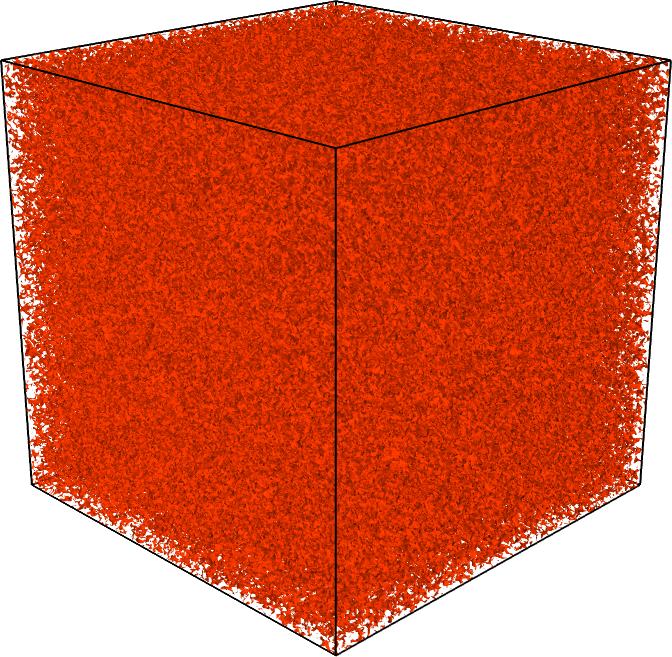
\includegraphics[width=0.35\linewidth]{numerics/figures/mess3d}%
    \begin{minipage}[b]{0.2\linewidth}
      \centering
      \raisebox{3cm}{$\longrightarrow$}
    \end{minipage}% 
    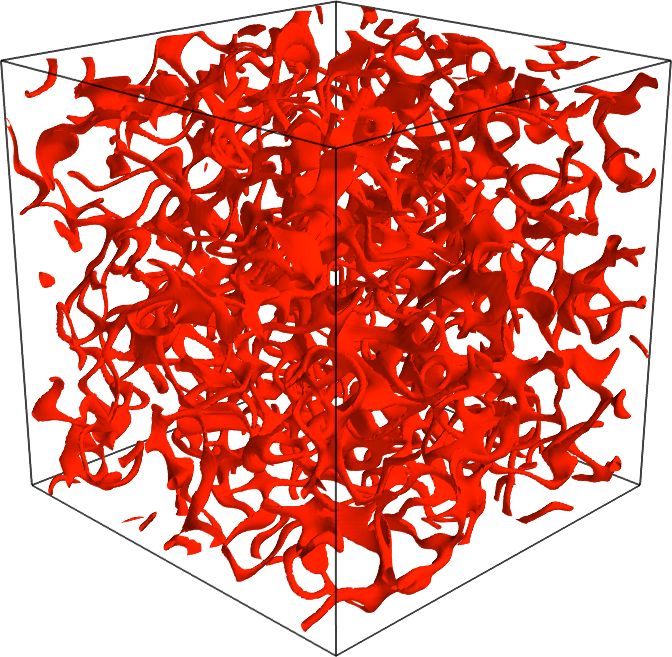
\includegraphics[width=0.35\linewidth]{numerics/figures/clean3d}
  \caption{(Left) Unfiltered wavefunction density, $|\psi|^2$, from a classical-field simulation with condensate fraction $\rho_0/\rho=0.22$ during equilibration. A vortex tangle is present but not visible by direct density visualisation. (Right) Filtered wavefunction density, $|\hat{\psi}|^2$, clearly showing the vortical structures in the gas.}\label{fig:quasicondensatefilter}
  \end{figure}

The choice of $k_c$ is facilitated by the the bimodal distribution of occupation numbers in the wavefunction, a distribution which develops naturally through propagation of the GPE. The high-$k$ part of the distribution is associated with the thermal excitations and low mode occupations. The low-$k$ part of the field is the quasi-condensate, characterised by macroscopic mode populations and superfluid ordering. $k_c$ is chosen as the boundary in $k$-space between the quasi-condensate and the thermal gas. Figure \ref{fig:quasicondensatefilter} demonstrates the filtering technique in action.

  	
\section{\label{section:linelength} Evaluation of vortex line-length in 3D}
For a given 3D wavefunction, $\Psi$, featuring a vortex distribution, the vortex volume $V_t$ (the total volume associated with the vortex cores) is evaluated by numerical integration of the inside of the vortex isosurface tubes obtained from the filtered density $|\hat \Psi|^2$, with an integration region of the whole numerical box.  Note that the isosurface level should be low enough to pick out vortex cores only (and not, e.g. fluctuations and waves), while large enough to contain sufficient grid points to allow a reasonable numerical evaluation of volume. In this work we use the isosurface level $0.04\langle |\hat{\Psi}|^2 \rangle$ (chosen so as to produce filtered vortex cores that are similar in radius to the true vortex core).  The volume calculation can be written $V_t = \int \Theta(0.04\langle |\hat{\Psi}|^2 \rangle - |\hat{\Psi}({\bf r})|^2)~{\rm d}V$, where $\Theta$ is the Heaviside step function. In practice the calculation of the vortex core volume can be efficiently performed by assigning a value of unity/zero to grid points located within/outside the isosurface tubes and directly integrating the result using the trapezium or Simpson's rule.

The total line length is then deduced by dividing $V_t$ by the cross-sectional area of a vortex core, $A_t$ (in effect, the average cross-sectional area of the isosurface tubes). The measured values of $V_t$ and $A_t$ will depend on the chosen isosurface level but, providing the vortex tubes are well-separated, their ratio (and hence the evaluated line length) will remain constant.  For closely-positioned vortex tubes, the isosurface level can affect whether the tubes appear as two separate tubes, or start to merge, and so will lead to deviations in this ratio.
\end{chapter}
